%% example on how to properly add a picture
% \begin{figure}[h]
%     \centering
%     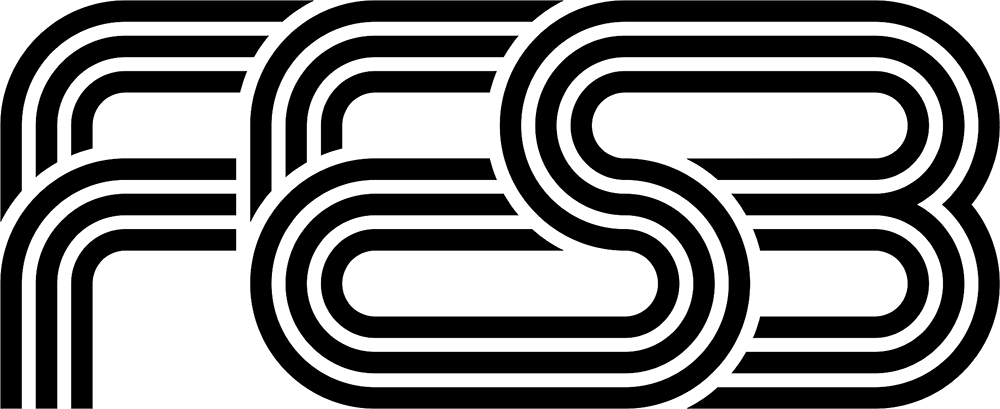
\includegraphics[scale=0.2]{fesb_logo.png}
%     \caption{An example graph}
%     \label{figure:fesb_logo}
% \end{figure}

Long Range Wide Area Network, or LoRaWAN for short, is a low power, media access control (MAC) protocol for wide area networks.
The LoRaWAN is often used in the Internet of Things (IoT) deployment, specially in a smart environment where there are thousands of end-devices (i.e. sensors) that require minimal bandwidth and consume low power.
The IoT is the extension of Internet connectivity into physical devices and everyday objects. 
The IoT, as an interconnection concept, serves, and will serve, variety of devices exchanging information about themselves and their surroundings.
Even though there are very few concrete definitons of the IoT, its classification can be defined strictly when it comes to the range. 
Three basic types of the IoT wireless networks, considering range, are:
\begin{itemize}
    \item short-range wireless IoT with commonly used communication protocols such as Bluetooth, Light-Fidelity, Near-field communication (NFC), Radio-frequency identification (RFID), Wi-Fi, ZigBee, etc.
    \item medium-range wireless IoT and the high-speed communication protocol for mobile networks LTE-Advanced
    \item long-range wireless IoT with protocols \textbf{Low-Power wide-area network} \\ (\textbf{LPWAN}) which is designed to allow long range communication at very low data rate thus reducing the power consumpiton and the overall cost of the transmission. There are a few widely used and relatively recent protocols: \textbf{LoRaWAN}, Sigfox, NB-IoT, Weigtless, RPMA.
\end{itemize}
An IoT device has limited memory, processing power and bandwidth and, most importantly, a low amount of available energy \cite{Aloys_LoRa}.
The core idea of the IoT is to maximize the lifetime of device's battery because by the end of 2020 there is expected to be over 50 bilion connected devices \cite{Evans_IoT}.
If the attitude of doing as much as possible with least amount of power consumed is taken as the most important in the IoT, it is easy to realize that standard cellular networks, as well as the WiFi technology are too \textit{power-hungry} and there is a strong need for using up-to-date technologies that fulfill the communication requirements of the IoT.

\section{LoRa technology overview}
LPWANs, unlike the traditional broadband, are not focused on enabling high data rates per device. 
Instead, the most important performance metrics are energy efficiency, scalability and coverage \cite{Mikhaylov_LoRaWAN}.

The current version of LPWAN is constructed as a cellular network consisted of the end devices (ED) and the base stations (BS). 
EDs are connected to and served by a BS thus forming a star-topology network around them, see fig. \ref{fig:lpwan}.
\begin{figure}[h]
    \centering
    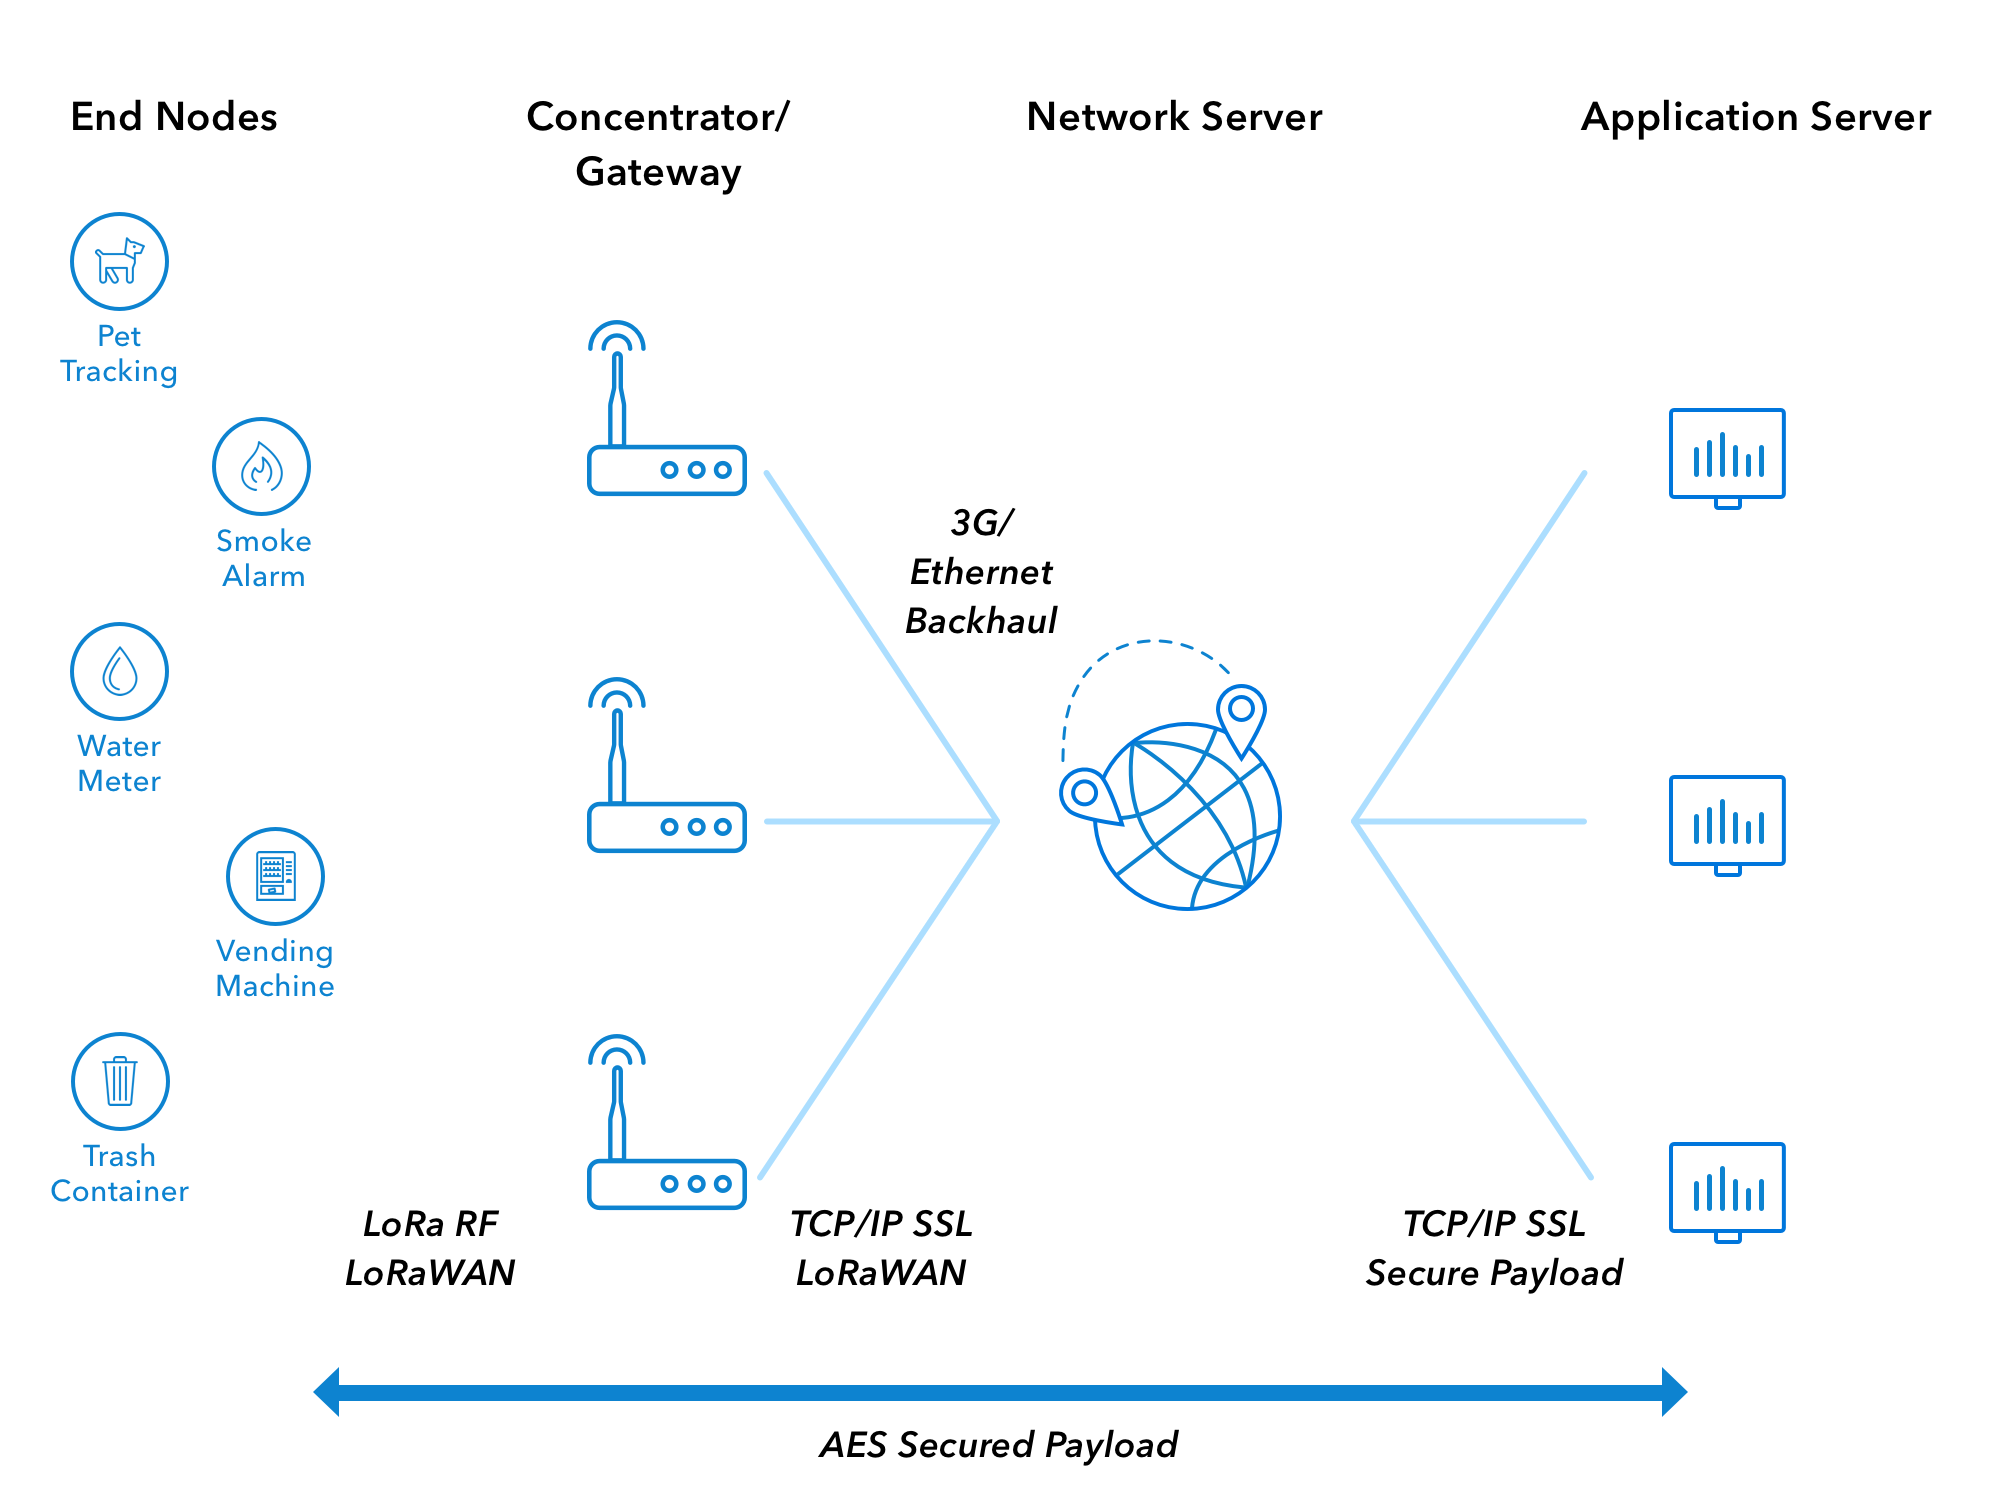
\includegraphics[width=\linewidth]{lpwan.png}
    \caption{An LPWAN as a star-of-stars topology network. Every end device is connected to a base station and every base station is connected to a central \textit{hub}, in this case to a network server \cite{TTN}.}
    \label{fig:lpwan}
\end{figure}

The most of the traffic in LPWANs is uplink where an ED communicates only to a BS and not with other EDs. A BS rarely sends any messages to an ED.

\textbf{LoRa} is the LPWAN protocol that targets deployments for already described environment (limited energy, low bandwidth, long range communication).
LoRa, as a long-range communication system, can refer to two distinct layers: \cite{Aloys_LoRa}
\begin{enumerate}
    \item a physical layer using the Chirp Spread Spectrum (CSS) modulation technique
    \item a media access control (MAC) layer protocol (LoRaWAN) 
\end{enumerate}
While the LoRaWAN is an open standard \cite{lora-alliance}, LoRa is a proprietary modulation technology based on the chirp spread spectrum developed and maintained by Semtech. 

\section{LoRa physical layer}
\subsection{Physical layer features}
The LoRa physical layer is a modulation based on the CSS scheme that uses wideband linear frequency modulated pulses whose frequency increases or decreases based on the encoded information \cite{Mikhaylov_LoRaWAN}.
Frequency offsets between the receiver and the transmitter are equivalent to timing offsets because of the linearity of the chirp and thus easily eliminated in the decoder. 
This also makes the LoRa modulation immune to the Doppler effect. 
Besides Doppler resistance, LoRa key properties are: long range connectivity, high robustness, multipath resistance, low power consumption \cite{Bor_LoRA}.

The CSS, as a modulation technique, is used to encode and transmit the data over large distances in the 868MHz band \cite{Reynders_CSS}. 
Chrip stands for Compressed High Intensity Radar Pulse and it is a signal which frequency, as mentioned, either increases (up-chirp) or decreases (down-chirp) with time.
Chirps are linear, which means that the frequency varies linearly with time:
\begin{equation}
    f(t) = f_{0} + kt
\end{equation}
where $ k $ is the slope of the chirp:
\begin{equation}
    k = \frac{f_{1} - f{0}}{T}
\end{equation}
The phase is described as:
$$ \theta (t) = \theta_{0} + 2\pi \int_{0}^{t}f(\tau)d\tau $$

$$ \theta (t) = \theta_{0} + 2\pi \int_{0}^{t}(f_{0} + kt) d\tau $$

\begin{equation}
    \theta(t) = \theta_{0} + 2\pi (f_{0}t + \frac{k}{2}t^{2})
\end{equation}
where $ \theta_{0} $ is the initial phase and $ f_{0} $ is the initial frequency.

There are several frequency bands LoRa can operate in, but the European frequeny band is defined in the 863-870 MHz range.
European regulations specify duty-cycles on devices for each sub-band.
The duty cycle indicates the fraction of time a resource is busy \cite{TTN}. 
Europen standards are defining the duty cycle at 1\% for most regions. 

\subsection{Parameters of the LoRa physical layer}
There are three key parameters for customization of the LoRa modulation:
\begin{itemize}
    \item bandwidth (BW) - the range of frequencies in the transmission band
    \item spreading factor (SF) - the ratio between the symbol rate and the chirp rate
    \item code rate (CR) - the FEC rate used by a modem to protect against the bursts and interferences
\end{itemize}
One LoRa symbol is composed of $ 2^{SF} $ chirps, which are spread all over the frequency band.
It starts with a preamble which is represented by a number of continuous up-chirps \cite{Knight}.
The last two and one forth chirps are the sync word after which the transmission of the actual payload begins, shown in fig. \ref{fig:lora_signal}.
\begin{figure}[h]
    \centering
    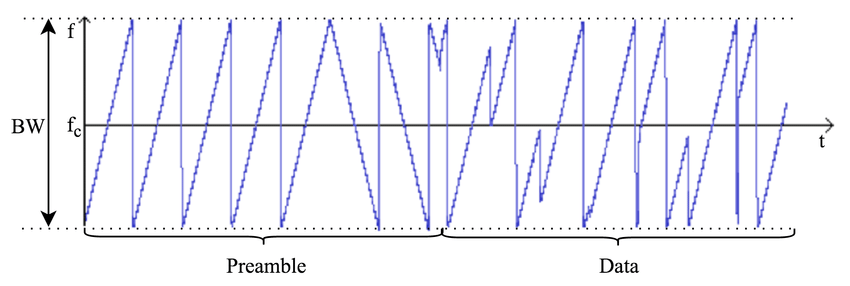
\includegraphics[width=\linewidth]{lora-signal.png}
    \caption{A frequency variation in time of a modulated signal emitted by a LoRa transmitter \cite{Aloys_LoRa}}
    \label{fig:lora_signal}
\end{figure}

As there are $ 2^{SF} $ chirps in a symbol, a symbol can effectively encode SF bits of information, where higher SF increases the signal-to-noise ratio (SNR) but also affects the air time of the packet.
From here, it is easy to derive the duration of the symbol regarding the spreading factor and the bandwidth:
\begin{equation}
    T_{s} = \frac{2^{SF}}{BW}
\end{equation}

Taking the relation of the code rate with the bandwidth and the spreading factor, and the fact that SF bits of information are transmitted per symbol, the useful bit rate is formulated with the equation:
\begin{equation}
    R_{b} = SF \times \frac{BW}{2^{SF}} \times CR 
\end{equation}

A data rate is a number of information bits that are conveyed per unit of time \cite{Silva_LoRaWAN}.
The adaptiveness should be enabled whenever the end device has stable RF conditions. 
The Adaptive Data Rate (ADR) optimizes the bit rate, the airtime and the energy consumption, and is affected mostly by the signal-to-noise ratio and the number of gateways that recevied each uplink message.

\subsection{Physical frame format}
A LoRa physical frame begins with a preamble. 
In fig. \ref{fig:lora_signal}, it is shown that the preamble starts with constant up-chirps that spread throughout the whole frequency band. The last two and one forth upchirps are the sync word which represents one byte value that is used to differentiate LoRa networks that use the same frequency band.
After the preamble, comes the optional header. The header is always configured with the code rate of 4/8.
The header indicates the size of the payload in bytes, the code rate used for the end of the transmission and wheter or not a 16-bit payload CRC is present in the frame \cite{Aloys_LoRa}.
If the information in a header is known in advance, there is no need to use a header.
The payload part of a frame is the actual data which size is limited on 255 bytes per frame.
After a payload, there is an optional cyclic redundancy checker on the end of the frame.
A frame is depicted in fig. \ref{fig:lora_phy_frame}.
\begin{figure}[h]
    \centering
    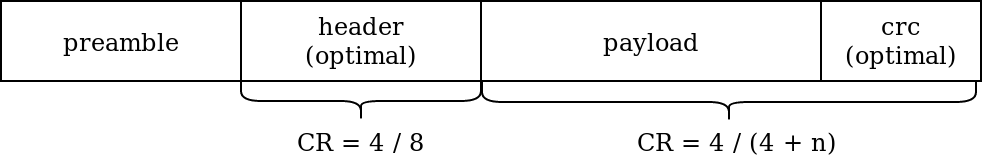
\includegraphics[width=\linewidth]{phy-frame.png}
    \caption{The structure of a LoRa frame}
    \label{fig:lora_phy_frame}
\end{figure}

The physical layer payload is consisted of elements defined in the official LoRaWAN specification from LoRa Alliance \cite{Sornin_LoRaWAN}.
The complete length of the physical layer payload is given by:
\begin{equation}
    PL = MHDR + MACPayload + MIC 
\end{equation}
where $MHDR=1$ is the length of the MAC header, $MACPayload$ is the media access control layer payload and $MIC=4$ is the message integrity code.
\begin{multline}
    PL = MHDR + FHDR_{ADDR} + FHDR_{FCTRL} +\\ FHDR_{CNT} + FHDR_{OPTS} + FPort + FRMPayload + MIC 
\end{multline}
where the payload of the MAC layer is consisted of $FHDR_{ADDR}=4$ which is the length of the ED address field of the frame header, lengths of the frame control $FHDR_{CNT}=4$ and the frame counter $FHDR_{FCTRL}=4$ fields and $FHDR_{OPTS}$, which is the length of the optional FHDR field carrying MAC commands.
$FPort=1$ is the application specific port identifier.
Taken all \textit{a priori} known lengths, the length of the physical layer payload is now:
\begin{equation}
    PL = 12 + FHDR_{OPTS} + FPORT + FRMPayload
\end{equation}

\section{Media access control layer}
\subsection{Devices and the network topology overview}
LoRaWAN is a media access control protocol built on top of LoRa and, unlike LoRa, is completely open sourced.
It is often used in the IoT deployment where end devices are simple rudimentary electronic devices with embedded sensors. 
End devices are expected to transmit packets to a base station using LoRa proprietary modulation with a low data rate using small bandwidth.
The LoRaWAN protocols are defined in \cite{Sornin_LoRaWAN}.
LoRaWAN architecture is based on a star-of-stars topology depicted in fig \ref{fig:lorawan}.
\begin{figure}[h]
    \centering
    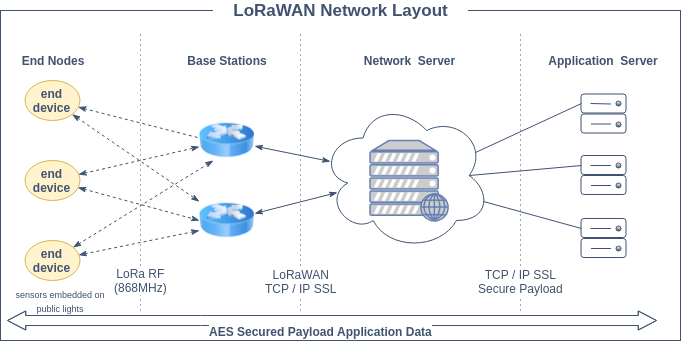
\includegraphics[width=\linewidth]{LoRaWAN-Network-Layout.png}
    \caption{Network topology of a typical LoRaWAN-based network. The communication is most often uplink, end devices send data to a base station which capture the MAC frames and dispatch them to a network server using a back-haul interface with high througput}
    \label{fig:lorawan}
\end{figure}
This architecure enables long range communication while keeping the device battery lifetime as long as possible.

There are three device types defined in the LoRaWAN specification:
\begin{description}
    \item[Class A devices] support bi-directional communication between the end device and the base station. Uplink message can be sent randomly, at any time. The end device opens two receiving windows RX1 and RX2 at specified times (1 second and 2 second respectively) after an uplink transmission. If there is no reply from the server during the duration of RX1 or RX2, the next opportunity to send data will happen after the next uplink transmission from the end device. Class A device mechanism is depicted in fig. \ref{fig:classA}.
    \item[Class B devices] extend the Class A functionality by adding scheduled receive windows for downlink traffic from the server.
    \item[Class C devices] behave similar to the Class A devices, but keep the receiving window continuosly open. They are at a high level of power consumption but achieve low-latency communication.
\end{description}
\begin{figure}[h]
    \centering
    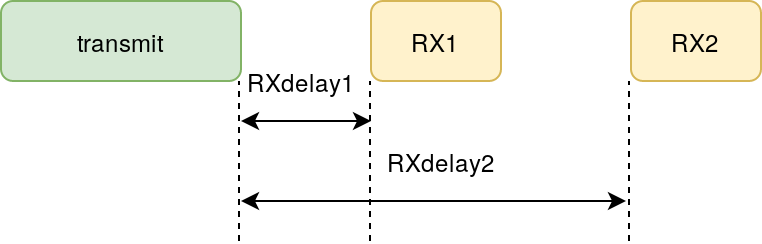
\includegraphics[width=0.7\linewidth]{classA.png}
    \caption{Class A device is commonly used device in the LoRaWAN deployment. RX1 and RX2 are receving windows enabled for server to respond but configured in a way that server should not use both RX windows}
    \label{fig:classA}
\end{figure}

LoRaWAN does not support device-to-device communication, packets can be transmitted only from an end device to a network server or, rarely, from a server to an end device.

\subsection{LoRaWAN message format}
Inside the payload section of the LoRa frame, depicted in fig. \ref{fig:lora_phy_frame} there are MAC header (MHDR), which indicates the type of MAC message, the MAC payload, which carries application data and the Message Integrity Code (MIC), which allows a receiver to check the integrity of a MAC message received.
The content of the MAC payload is the frame header (FHDR), the frame port (FPort) and the frame payload \cite{ibanez_lorawan}. 
The LoRaWAN media access control message format is shown in fig. \ref{fig:lora_mac_frame}.
\begin{figure}[h]
    \centering
    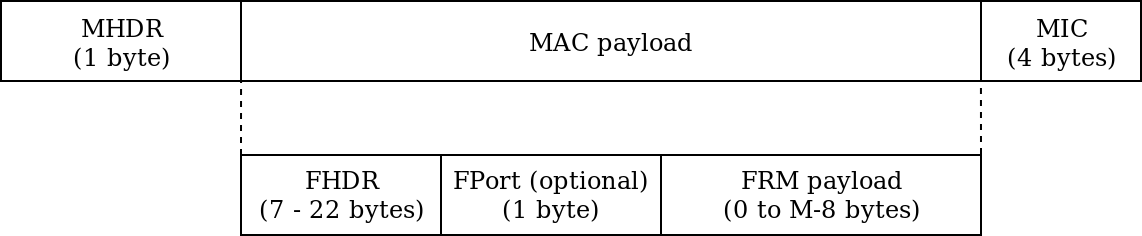
\includegraphics[width=\linewidth]{lora-mac-frame.png}
    \caption{LoRaWAN MAC message format. The FPort field is present when the frame payload field contains data (has non-zero length). $M$ is the maximum size of the MAC Payload field. The frame header (FHDR) field has a size of 7 bytes if it does not contain options, and up to 22 bytes when options are used.}
    \label{fig:lora_mac_frame}
\end{figure}

FHDR is consited of:
\begin{itemize}
    \item DevAddr -- 4 bytes end device address
    \item FCtrl -- 1 byte frame control further consisted of different flags for uplink and downlink messages
    \item FCnt -- 2 bytes frame counter
    \item FOpts -- use to piggyback MAC commands on a data message
\end{itemize}

The minimal size of the MAC header is 13 bytes while the maximal size is 28 bytes.

\subsection{Network setup and security}
To deploy a LoRaWAN network, it is important to activate end devices. 
All LoRaWAN devices have a 64 bit unique device identifier (DevEUI) that is assigned by the chip manufacturer.
Communication is done using 32 bit device address (DevAddr) where the first 7 bits are dedicated for the hosting network and 25 bits are left to be assigned to individual devices. 
The assignment of the DevAddr identifier is done through an activation procedure. 
There are two basic ways to activate the end device: \cite{TTN}
\begin{itemize}
    \item Over-The-Air Activation (OTAA) -- more secure way to connect in which devices perform a join-procedure with the network (negotiation of security keys)
    \item Activation By Personalization (ABP) -- hardcoding the DevAddr to the end device
\end{itemize}

Other than DevAddr, during the activation procedure the following information should be inquired by the end device: \cite{Aloys_LoRa}
\begin{itemize}
    \item application identifier (AppEUI) -- a global application ID that identifies the owner of the end device
    \item network session key (NwkSKey) -- a key used by the network server and the end device to verify the MIC of all data to ensure data integrity
    \item application session key (AppSKey) -- a key used by the network server and the end device to encrypt and decrypt the payload field of data messages
\end{itemize}

The extensive view on the security and the security challenges of LoRaWAN is given in \cite{security_lora}. Here, only key features and possible improvements will be presented.
The LoRaWAN utilizes two layers of security: one for the network and one for the application layer. 
The network layer security is responsible for the authenticity of the end device in the network, while the application layer security makes sure that the network operator does not have access to the actual content of the MAC payload.
The process of the end device activation is marked with secure keys exchange. 
Two session keys (NwkSKey and AppSKey) are unique to each device and to each session. 
If a device is dynamically activated via the OTAA activation, keys will be generated again with each new activation. 
If the end device is statically activated through the ABP activation process, secure keys are hardcoded and stay the same with each activation.
LoRaWAN systems come with end-to-end data confidentiality and integrity that should be manufacturer and network provider agnostic. 
The encryption with the key exchange implemented in the LoRaWAN is the Advanced Encryption Standard (AES), based on the security for IEEE 802.15.4 wireless networks.
Even though the LoRaWAN provides an end-to-end security both through the network security layer and the application security layer, there are still few weaknesses of the security features in the LoRaWAN standard.
Firstly, encrypted messages have the same length as the key. Secondly, if the session keys are compromised, security will be rendered ineffective as it would be too complex to change the AES keys on all nodes and devices. 
Moreover, the session keys (AppKey, NwkSKey and AppSKey) are a big issue. 
Lastly, identification and connection processes could be a huge weakness. 
All base stations send their personal IDs (beacons) periodically to the server. 
It is fairly easy for the attackers to obtain this ID, which can be used for overriding the base station.